\documentclass[1p]{elsarticle_modified}
%\bibliographystyle{elsarticle-num}

%\usepackage[colorlinks]{hyperref}
%\usepackage{abbrmath_seonhwa} %\Abb, \Ascr, \Acal ,\Abf, \Afrak
\usepackage{amsfonts}
\usepackage{amssymb}
\usepackage{amsmath}
\usepackage{amsthm}
\usepackage{scalefnt}
\usepackage{amsbsy}
\usepackage{kotex}
\usepackage{caption}
\usepackage{subfig}
\usepackage{color}
\usepackage{graphicx}
\usepackage{xcolor} %% white, black, red, green, blue, cyan, magenta, yellow
\usepackage{float}
\usepackage{setspace}
\usepackage{hyperref}

\usepackage{tikz}
\usetikzlibrary{arrows}

\usepackage{multirow}
\usepackage{array} % fixed length table
\usepackage{hhline}

%%%%%%%%%%%%%%%%%%%%%
\makeatletter
\renewcommand*\env@matrix[1][\arraystretch]{%
	\edef\arraystretch{#1}%
	\hskip -\arraycolsep
	\let\@ifnextchar\new@ifnextchar
	\array{*\c@MaxMatrixCols c}}
\makeatother %https://tex.stackexchange.com/questions/14071/how-can-i-increase-the-line-spacing-in-a-matrix
%%%%%%%%%%%%%%%

\usepackage[normalem]{ulem}

\newcommand{\msout}[1]{\ifmmode\text{\sout{\ensuremath{#1}}}\else\sout{#1}\fi}
%SOURCE: \msout is \stkout macro in https://tex.stackexchange.com/questions/20609/strikeout-in-math-mode

\newcommand{\cancel}[1]{
	\ifmmode
	{\color{red}\msout{#1}}
	\else
	{\color{red}\sout{#1}}
	\fi
}

\newcommand{\add}[1]{
	{\color{blue}\uwave{#1}}
}

\newcommand{\replace}[2]{
	\ifmmode
	{\color{red}\msout{#1}}{\color{blue}\uwave{#2}}
	\else
	{\color{red}\sout{#1}}{\color{blue}\uwave{#2}}
	\fi
}

\newcommand{\Sol}{\mathcal{S}} %segment
\newcommand{\D}{D} %diagram
\newcommand{\A}{\mathcal{A}} %arc


%%%%%%%%%%%%%%%%%%%%%%%%%%%%%5 test

\def\sl{\operatorname{\textup{SL}}(2,\Cbb)}
\def\psl{\operatorname{\textup{PSL}}(2,\Cbb)}
\def\quan{\mkern 1mu \triangleright \mkern 1mu}

\theoremstyle{definition}
\newtheorem{thm}{Theorem}[section]
\newtheorem{prop}[thm]{Proposition}
\newtheorem{lem}[thm]{Lemma}
\newtheorem{ques}[thm]{Question}
\newtheorem{cor}[thm]{Corollary}
\newtheorem{defn}[thm]{Definition}
\newtheorem{exam}[thm]{Example}
\newtheorem{rmk}[thm]{Remark}
\newtheorem{alg}[thm]{Algorithm}

\newcommand{\I}{\sqrt{-1}}
\begin{document}

%\begin{frontmatter}
%
%\title{Boundary parabolic representations of knots up to 8 crossings}
%
%%% Group authors per affiliation:
%\author{Yunhi Cho} 
%\address{Department of Mathematics, University of Seoul, Seoul, Korea}
%\ead{yhcho@uos.ac.kr}
%
%
%\author{Seonhwa Kim} %\fnref{s_kim}}
%\address{Center for Geometry and Physics, Institute for Basic Science, Pohang, 37673, Korea}
%\ead{ryeona17@ibs.re.kr}
%
%\author{Hyuk Kim}
%\address{Department of Mathematical Sciences, Seoul National University, Seoul 08826, Korea}
%\ead{hyukkim@snu.ac.kr}
%
%\author{Seokbeom Yoon}
%\address{Department of Mathematical Sciences, Seoul National University, Seoul, 08826,  Korea}
%\ead{sbyoon15@snu.ac.kr}
%
%\begin{abstract}
%We find all boundary parabolic representation of knots up to 8 crossings.
%
%\end{abstract}
%\begin{keyword}
%    \MSC[2010] 57M25 
%\end{keyword}
%
%\end{frontmatter}

%\linenumbers
%\tableofcontents
%
\newcommand\colored[1]{\textcolor{white}{\rule[-0.35ex]{0.8em}{1.4ex}}\kern-0.8em\color{red} #1}%
%\newcommand\colored[1]{\textcolor{white}{ #1}\kern-2.17ex	\textcolor{white}{ #1}\kern-1.81ex	\textcolor{white}{ #1}\kern-2.15ex\color{red}#1	}

{\Large $\underline{12n_{0170}~(K12n_{0170})}$}

\setlength{\tabcolsep}{10pt}
\renewcommand{\arraystretch}{1.6}
\vspace{1cm}\begin{tabular}{m{100pt}>{\centering\arraybackslash}m{274pt}}
\multirow{5}{120pt}{
	\centering
	\includegraphics[width=112pt]{../../../GIT/diagram.site/Diagrams/png/2259_12n_0170.png}\\
\ \ \ A knot diagram\footnotemark}&
\allowdisplaybreaks
\textbf{Linearized knot diagam} \\
\cline{2-2}
 &
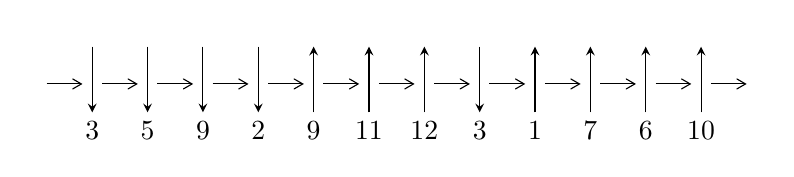
\begin{tikzpicture}[x=20pt, y=17pt]
	% nodes
	\node (C0) at (0, 0) {};
	\node (C1) at (1, 0) {};
	\node (C1U) at (1, +1) {};
	\node (C1D) at (1, -1) {3};

	\node (C2) at (2, 0) {};
	\node (C2U) at (2, +1) {};
	\node (C2D) at (2, -1) {5};

	\node (C3) at (3, 0) {};
	\node (C3U) at (3, +1) {};
	\node (C3D) at (3, -1) {9};

	\node (C4) at (4, 0) {};
	\node (C4U) at (4, +1) {};
	\node (C4D) at (4, -1) {2};

	\node (C5) at (5, 0) {};
	\node (C5U) at (5, +1) {};
	\node (C5D) at (5, -1) {9};

	\node (C6) at (6, 0) {};
	\node (C6U) at (6, +1) {};
	\node (C6D) at (6, -1) {11};

	\node (C7) at (7, 0) {};
	\node (C7U) at (7, +1) {};
	\node (C7D) at (7, -1) {12};

	\node (C8) at (8, 0) {};
	\node (C8U) at (8, +1) {};
	\node (C8D) at (8, -1) {3};

	\node (C9) at (9, 0) {};
	\node (C9U) at (9, +1) {};
	\node (C9D) at (9, -1) {1};

	\node (C10) at (10, 0) {};
	\node (C10U) at (10, +1) {};
	\node (C10D) at (10, -1) {7};

	\node (C11) at (11, 0) {};
	\node (C11U) at (11, +1) {};
	\node (C11D) at (11, -1) {6};

	\node (C12) at (12, 0) {};
	\node (C12U) at (12, +1) {};
	\node (C12D) at (12, -1) {10};
	\node (C13) at (13, 0) {};

	% arrows
	\draw[->,>={angle 60}]
	(C0) edge (C1) (C1) edge (C2) (C2) edge (C3) (C3) edge (C4) (C4) edge (C5) (C5) edge (C6) (C6) edge (C7) (C7) edge (C8) (C8) edge (C9) (C9) edge (C10) (C10) edge (C11) (C11) edge (C12) (C12) edge (C13) ;	\draw[->,>=stealth]
	(C1U) edge (C1D) (C2U) edge (C2D) (C3U) edge (C3D) (C4U) edge (C4D) (C5D) edge (C5U) (C6D) edge (C6U) (C7D) edge (C7U) (C8U) edge (C8D) (C9D) edge (C9U) (C10D) edge (C10U) (C11D) edge (C11U) (C12D) edge (C12U) ;
	\end{tikzpicture} \\
\hhline{~~} \\& 
\textbf{Solving Sequence} \\ \cline{2-2} 
 &
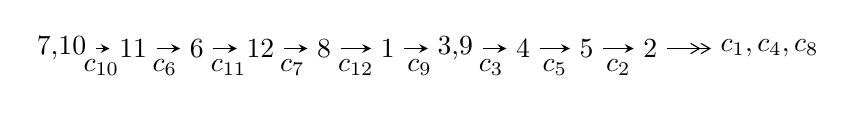
\begin{tikzpicture}[x=23pt, y=7pt]
	% node
	\node (A0) at (-1/8, 0) {7,10};
	\node (A1) at (1, 0) {11};
	\node (A2) at (2, 0) {6};
	\node (A3) at (3, 0) {12};
	\node (A4) at (4, 0) {8};
	\node (A5) at (5, 0) {1};
	\node (A6) at (97/16, 0) {3,9};
	\node (A7) at (57/8, 0) {4};
	\node (A8) at (65/8, 0) {5};
	\node (A9) at (73/8, 0) {2};
	\node (C1) at (1/2, -1) {$c_{10}$};
	\node (C2) at (3/2, -1) {$c_{6}$};
	\node (C3) at (5/2, -1) {$c_{11}$};
	\node (C4) at (7/2, -1) {$c_{7}$};
	\node (C5) at (9/2, -1) {$c_{12}$};
	\node (C6) at (11/2, -1) {$c_{9}$};
	\node (C7) at (53/8, -1) {$c_{3}$};
	\node (C8) at (61/8, -1) {$c_{5}$};
	\node (C9) at (69/8, -1) {$c_{2}$};
	\node (A10) at (11, 0) {$c_{1},c_{4},c_{8}$};

	% edge
	\draw[->,>=stealth]	
	(A0) edge (A1) (A1) edge (A2) (A2) edge (A3) (A3) edge (A4) (A4) edge (A5) (A5) edge (A6) (A6) edge (A7) (A7) edge (A8) (A8) edge (A9) ;
	\draw[->>,>={angle 60}]	
	(A9) edge (A10);
\end{tikzpicture} \\ 

\end{tabular} \\

\footnotetext{
The image of knot diagram is generated by the software ``\textbf{Draw programme}" developed by Andrew Bartholomew(\url{http://www.layer8.co.uk/maths/draw/index.htm\#Running-draw}), where we modified some parts for our purpose(\url{https://github.com/CATsTAILs/LinksPainter}).
}\phantom \\ \newline 
\centering \textbf{Ideals for irreducible components\footnotemark of $X_{\text{par}}$} 
 
\begin{align*}
I^u_{1}&=\langle 
-2 u^{46}+4 u^{45}+\cdots+b+2,\;2 u^{45}-2 u^{44}+\cdots+a-1,\;u^{47}-2 u^{46}+\cdots-12 u^2+1\rangle \\
I^u_{2}&=\langle 
b- u,\;a- u-1,\;u^3+2 u-1\rangle \\
I^u_{3}&=\langle 
u^3+b+2 u+1,\;a+1,\;u^4+u^3+2 u^2+2 u+1\rangle \\
\\
\end{align*}
\raggedright * 3 irreducible components of $\dim_{\mathbb{C}}=0$, with total 54 representations.\\
\footnotetext{All coefficients of polynomials are rational numbers. But the coefficients are sometimes approximated in decimal forms when there is not enough margin.}
\newpage
\renewcommand{\arraystretch}{1}
\centering \section*{I. $I^u_{1}= \langle -2 u^{46}+4 u^{45}+\cdots+b+2,\;2 u^{45}-2 u^{44}+\cdots+a-1,\;u^{47}-2 u^{46}+\cdots-12 u^2+1 \rangle$}
\flushleft \textbf{(i) Arc colorings}\\
\begin{tabular}{m{7pt} m{180pt} m{7pt} m{180pt} }
\flushright $a_{7}=$&$\begin{pmatrix}0\\u\end{pmatrix}$ \\
\flushright $a_{10}=$&$\begin{pmatrix}1\\0\end{pmatrix}$ \\
\flushright $a_{11}=$&$\begin{pmatrix}1\\- u^2\end{pmatrix}$ \\
\flushright $a_{6}=$&$\begin{pmatrix}- u\\u^3+u\end{pmatrix}$ \\
\flushright $a_{12}=$&$\begin{pmatrix}u^2+1\\- u^4-2 u^2\end{pmatrix}$ \\
\flushright $a_{8}=$&$\begin{pmatrix}u^5+2 u^3+u\\- u^7-3 u^5-2 u^3+u\end{pmatrix}$ \\
\flushright $a_{1}=$&$\begin{pmatrix}- u^4- u^2+1\\- u^4-2 u^2\end{pmatrix}$ \\
\flushright $a_{3}=$&$\begin{pmatrix}-2 u^{45}+2 u^{44}+\cdots-5 u+1\\2 u^{46}-4 u^{45}+\cdots-3 u-2\end{pmatrix}$ \\
\flushright $a_{9}=$&$\begin{pmatrix}u^8+3 u^6+u^4-2 u^2+1\\u^8+4 u^6+4 u^4\end{pmatrix}$ \\
\flushright $a_{4}=$&$\begin{pmatrix}-4 u^{45}+4 u^{44}+\cdots+16 u^2-5 u\\4 u^{46}-8 u^{45}+\cdots-4 u-4\end{pmatrix}$ \\
\flushright $a_{5}=$&$\begin{pmatrix}- u^{19}-8 u^{17}-24 u^{15}-30 u^{13}-7 u^{11}+10 u^9-4 u^7-6 u^5+3 u^3-2 u\\- u^{19}-9 u^{17}-32 u^{15}-55 u^{13}-43 u^{11}-9 u^9-4 u^5+u^3+u\end{pmatrix}$ \\
\flushright $a_{2}=$&$\begin{pmatrix}- u^{45}+u^{44}+\cdots-4 u+2\\u^{46}-2 u^{45}+\cdots-2 u-1\end{pmatrix}$\\&\end{tabular}
\flushleft \textbf{(ii) Obstruction class $= -1$}\\~\\
\flushleft \textbf{(iii) Cusp Shapes $= -4 u^{46}+8 u^{45}+\cdots+38 u+5$}\\~\\
\newpage\renewcommand{\arraystretch}{1}
\flushleft \textbf{(iv) u-Polynomials at the component}\newline \\
\begin{tabular}{m{50pt}|m{274pt}}
Crossings & \hspace{64pt}u-Polynomials at each crossing \\
\hline $$\begin{aligned}c_{1}\end{aligned}$$&$\begin{aligned}
&u^{47}+14 u^{46}+\cdots-5 u+1
\end{aligned}$\\
\hline $$\begin{aligned}c_{2},c_{4}\end{aligned}$$&$\begin{aligned}
&u^{47}-8 u^{46}+\cdots-5 u+1
\end{aligned}$\\
\hline $$\begin{aligned}c_{3},c_{8}\end{aligned}$$&$\begin{aligned}
&u^{47}+u^{46}+\cdots+192 u+128
\end{aligned}$\\
\hline $$\begin{aligned}c_{5}\end{aligned}$$&$\begin{aligned}
&u^{47}-2 u^{46}+\cdots+2 u+1
\end{aligned}$\\
\hline $$\begin{aligned}c_{6},c_{10},c_{11}\end{aligned}$$&$\begin{aligned}
&u^{47}-2 u^{46}+\cdots-12 u^2+1
\end{aligned}$\\
\hline $$\begin{aligned}c_{7}\end{aligned}$$&$\begin{aligned}
&u^{47}+2 u^{46}+\cdots+96 u+72
\end{aligned}$\\
\hline $$\begin{aligned}c_{9},c_{12}\end{aligned}$$&$\begin{aligned}
&u^{47}+8 u^{46}+\cdots+112 u-49
\end{aligned}$\\
\hline
\end{tabular}\\~\\
\newpage\renewcommand{\arraystretch}{1}
\flushleft \textbf{(v) Riley Polynomials at the component}\newline \\
\begin{tabular}{m{50pt}|m{274pt}}
Crossings & \hspace{64pt}Riley Polynomials at each crossing \\
\hline $$\begin{aligned}c_{1}\end{aligned}$$&$\begin{aligned}
&y^{47}+46 y^{46}+\cdots+83 y-1
\end{aligned}$\\
\hline $$\begin{aligned}c_{2},c_{4}\end{aligned}$$&$\begin{aligned}
&y^{47}-14 y^{46}+\cdots-5 y-1
\end{aligned}$\\
\hline $$\begin{aligned}c_{3},c_{8}\end{aligned}$$&$\begin{aligned}
&y^{47}+45 y^{46}+\cdots-167936 y-16384
\end{aligned}$\\
\hline $$\begin{aligned}c_{5}\end{aligned}$$&$\begin{aligned}
&y^{47}-52 y^{46}+\cdots+24 y-1
\end{aligned}$\\
\hline $$\begin{aligned}c_{6},c_{10},c_{11}\end{aligned}$$&$\begin{aligned}
&y^{47}+44 y^{46}+\cdots+24 y-1
\end{aligned}$\\
\hline $$\begin{aligned}c_{7}\end{aligned}$$&$\begin{aligned}
&y^{47}+12 y^{46}+\cdots+50832 y-5184
\end{aligned}$\\
\hline $$\begin{aligned}c_{9},c_{12}\end{aligned}$$&$\begin{aligned}
&y^{47}+32 y^{46}+\cdots+170128 y-2401
\end{aligned}$\\
\hline
\end{tabular}\\~\\
\newpage\flushleft \textbf{(vi) Complex Volumes and Cusp Shapes}
$$\begin{array}{c|c|c}  
\text{Solutions to }I^u_{1}& \I (\text{vol} + \sqrt{-1}CS) & \text{Cusp shape}\\
 \hline 
\begin{aligned}
u &= -0.240850 + 1.172380 I \\
a &= \phantom{-}0.76218 + 1.23522 I \\
b &= \phantom{-}0.934577 + 0.402639 I\end{aligned}
 & \phantom{-}4.61957 - 0.02295 I & \phantom{-0.000000 } 0 \\ \hline\begin{aligned}
u &= -0.240850 - 1.172380 I \\
a &= \phantom{-}0.76218 - 1.23522 I \\
b &= \phantom{-}0.934577 - 0.402639 I\end{aligned}
 & \phantom{-}4.61957 + 0.02295 I & \phantom{-0.000000 } 0 \\ \hline\begin{aligned}
u &= \phantom{-}0.708507 + 0.363703 I \\
a &= -0.94806 + 1.22755 I \\
b &= \phantom{-}2.37910 + 1.16766 I\end{aligned}
 & \phantom{-}3.42438 + 9.90306 I & \phantom{-}2.22004 - 7.67510 I \\ \hline\begin{aligned}
u &= \phantom{-}0.708507 - 0.363703 I \\
a &= -0.94806 - 1.22755 I \\
b &= \phantom{-}2.37910 - 1.16766 I\end{aligned}
 & \phantom{-}3.42438 - 9.90306 I & \phantom{-}2.22004 + 7.67510 I \\ \hline\begin{aligned}
u &= -0.635055 + 0.455943 I \\
a &= \phantom{-}0.114980 + 0.251136 I \\
b &= \phantom{-}0.0894725 + 0.0904282 I\end{aligned}
 & -4.12081 - 2.09104 I & \phantom{-}4.57556 + 3.64684 I \\ \hline\begin{aligned}
u &= -0.635055 - 0.455943 I \\
a &= \phantom{-}0.114980 - 0.251136 I \\
b &= \phantom{-}0.0894725 - 0.0904282 I\end{aligned}
 & -4.12081 + 2.09104 I & \phantom{-}4.57556 - 3.64684 I \\ \hline\begin{aligned}
u &= \phantom{-}0.517341 + 0.581926 I \\
a &= -1.35583 - 1.46783 I \\
b &= -1.70532 + 1.15194 I\end{aligned}
 & \phantom{-}2.58809 - 5.73384 I & \phantom{-}0.56569 + 2.04831 I \\ \hline\begin{aligned}
u &= \phantom{-}0.517341 - 0.581926 I \\
a &= -1.35583 + 1.46783 I \\
b &= -1.70532 - 1.15194 I\end{aligned}
 & \phantom{-}2.58809 + 5.73384 I & \phantom{-}0.56569 - 2.04831 I \\ \hline\begin{aligned}
u &= \phantom{-}0.109843 + 1.219880 I \\
a &= \phantom{-}0.767710 + 0.740963 I \\
b &= \phantom{-}0.864402 + 0.041075 I\end{aligned}
 & -2.27528 + 2.11283 I & \phantom{-0.000000 } 0 \\ \hline\begin{aligned}
u &= \phantom{-}0.109843 - 1.219880 I \\
a &= \phantom{-}0.767710 - 0.740963 I \\
b &= \phantom{-}0.864402 - 0.041075 I\end{aligned}
 & -2.27528 - 2.11283 I & \phantom{-0.000000 } 0\\
 \hline 
 \end{array}$$\newpage$$\begin{array}{c|c|c}  
\text{Solutions to }I^u_{1}& \I (\text{vol} + \sqrt{-1}CS) & \text{Cusp shape}\\
 \hline 
\begin{aligned}
u &= \phantom{-}0.698777 + 0.324988 I \\
a &= \phantom{-}1.001160 - 0.887981 I \\
b &= -2.00444 - 1.18278 I\end{aligned}
 & \phantom{-}4.64870 + 3.20376 I & \phantom{-}4.16524 - 3.31906 I \\ \hline\begin{aligned}
u &= \phantom{-}0.698777 - 0.324988 I \\
a &= \phantom{-}1.001160 + 0.887981 I \\
b &= -2.00444 + 1.18278 I\end{aligned}
 & \phantom{-}4.64870 - 3.20376 I & \phantom{-}4.16524 + 3.31906 I \\ \hline\begin{aligned}
u &= -0.256980 + 1.225330 I \\
a &= -0.62010 - 1.29363 I \\
b &= -0.881559 - 0.519345 I\end{aligned}
 & \phantom{-}4.25025 - 6.95397 I & \phantom{-0.000000 } 0 \\ \hline\begin{aligned}
u &= -0.256980 - 1.225330 I \\
a &= -0.62010 + 1.29363 I \\
b &= -0.881559 + 0.519345 I\end{aligned}
 & \phantom{-}4.25025 + 6.95397 I & \phantom{-0.000000 } 0 \\ \hline\begin{aligned}
u &= \phantom{-}0.435156 + 0.599476 I \\
a &= \phantom{-}1.31533 + 1.27222 I \\
b &= \phantom{-}1.34439 - 0.94929 I\end{aligned}
 & \phantom{-}3.57234 + 0.73807 I & \phantom{-}1.82651 - 2.67731 I \\ \hline\begin{aligned}
u &= \phantom{-}0.435156 - 0.599476 I \\
a &= \phantom{-}1.31533 - 1.27222 I \\
b &= \phantom{-}1.34439 + 0.94929 I\end{aligned}
 & \phantom{-}3.57234 - 0.73807 I & \phantom{-}1.82651 + 2.67731 I \\ \hline\begin{aligned}
u &= -0.037205 + 1.270570 I \\
a &= -1.61889 - 0.61214 I \\
b &= -1.283830 + 0.388483 I\end{aligned}
 & -4.85814 - 0.97601 I & \phantom{-0.000000 } 0 \\ \hline\begin{aligned}
u &= -0.037205 - 1.270570 I \\
a &= -1.61889 + 0.61214 I \\
b &= -1.283830 - 0.388483 I\end{aligned}
 & -4.85814 + 0.97601 I & \phantom{-0.000000 } 0 \\ \hline\begin{aligned}
u &= -0.623399 + 0.342153 I \\
a &= -0.426734 + 0.510909 I \\
b &= -0.111541 + 0.262625 I\end{aligned}
 & -1.47489 - 3.82342 I & \phantom{-}0.98515 + 6.99857 I \\ \hline\begin{aligned}
u &= -0.623399 - 0.342153 I \\
a &= -0.426734 - 0.510909 I \\
b &= -0.111541 - 0.262625 I\end{aligned}
 & -1.47489 + 3.82342 I & \phantom{-}0.98515 - 6.99857 I\\
 \hline 
 \end{array}$$\newpage$$\begin{array}{c|c|c}  
\text{Solutions to }I^u_{1}& \I (\text{vol} + \sqrt{-1}CS) & \text{Cusp shape}\\
 \hline 
\begin{aligned}
u &= -0.701377 + 0.026834 I \\
a &= -0.073148 + 1.342220 I \\
b &= -0.017726 + 0.554191 I\end{aligned}
 & \phantom{-}8.08746 - 3.45650 I & \phantom{-}7.23123 + 2.83028 I \\ \hline\begin{aligned}
u &= -0.701377 - 0.026834 I \\
a &= -0.073148 - 1.342220 I \\
b &= -0.017726 - 0.554191 I\end{aligned}
 & \phantom{-}8.08746 + 3.45650 I & \phantom{-}7.23123 - 2.83028 I \\ \hline\begin{aligned}
u &= \phantom{-}0.568091 + 0.371758 I \\
a &= -2.10914 - 0.10547 I \\
b &= \phantom{-}0.57523 + 2.44925 I\end{aligned}
 & -3.30787 + 1.75612 I & \phantom{-}1.06262 - 3.54613 I \\ \hline\begin{aligned}
u &= \phantom{-}0.568091 - 0.371758 I \\
a &= -2.10914 + 0.10547 I \\
b &= \phantom{-}0.57523 - 2.44925 I\end{aligned}
 & -3.30787 - 1.75612 I & \phantom{-}1.06262 + 3.54613 I \\ \hline\begin{aligned}
u &= \phantom{-}0.155614 + 1.341930 I \\
a &= -0.415404 + 0.937335 I \\
b &= \phantom{-}0.224512 + 0.844236 I\end{aligned}
 & -3.43598 + 2.59417 I & \phantom{-0.000000 } 0 \\ \hline\begin{aligned}
u &= \phantom{-}0.155614 - 1.341930 I \\
a &= -0.415404 - 0.937335 I \\
b &= \phantom{-}0.224512 - 0.844236 I\end{aligned}
 & -3.43598 - 2.59417 I & \phantom{-0.000000 } 0 \\ \hline\begin{aligned}
u &= -0.480171 + 0.404521 I \\
a &= \phantom{-}0.848787 - 0.023160 I \\
b &= \phantom{-}0.311223 - 0.154426 I\end{aligned}
 & -1.96248 + 0.31457 I & -1.52612 + 0.64426 I \\ \hline\begin{aligned}
u &= -0.480171 - 0.404521 I \\
a &= \phantom{-}0.848787 + 0.023160 I \\
b &= \phantom{-}0.311223 + 0.154426 I\end{aligned}
 & -1.96248 - 0.31457 I & -1.52612 - 0.64426 I \\ \hline\begin{aligned}
u &= -0.19689 + 1.43311 I \\
a &= -0.446867 + 0.559009 I \\
b &= -0.063667 + 0.550788 I\end{aligned}
 & -7.79399 - 2.25837 I & \phantom{-0.000000 } 0 \\ \hline\begin{aligned}
u &= -0.19689 - 1.43311 I \\
a &= -0.446867 - 0.559009 I \\
b &= -0.063667 - 0.550788 I\end{aligned}
 & -7.79399 + 2.25837 I & \phantom{-0.000000 } 0\\
 \hline 
 \end{array}$$\newpage$$\begin{array}{c|c|c}  
\text{Solutions to }I^u_{1}& \I (\text{vol} + \sqrt{-1}CS) & \text{Cusp shape}\\
 \hline 
\begin{aligned}
u &= \phantom{-}0.12786 + 1.44594 I \\
a &= -1.76062 + 0.79907 I \\
b &= -0.81689 + 1.44748 I\end{aligned}
 & -2.88567 + 2.62103 I & \phantom{-0.000000 } 0 \\ \hline\begin{aligned}
u &= \phantom{-}0.12786 - 1.44594 I \\
a &= -1.76062 - 0.79907 I \\
b &= -0.81689 - 1.44748 I\end{aligned}
 & -2.88567 - 2.62103 I & \phantom{-0.000000 } 0 \\ \hline\begin{aligned}
u &= -0.23877 + 1.43350 I \\
a &= \phantom{-}0.045007 - 0.588992 I \\
b &= -0.205747 - 0.403699 I\end{aligned}
 & -7.17228 - 6.98944 I & \phantom{-0.000000 } 0 \\ \hline\begin{aligned}
u &= -0.23877 - 1.43350 I \\
a &= \phantom{-}0.045007 + 0.588992 I \\
b &= -0.205747 + 0.403699 I\end{aligned}
 & -7.17228 + 6.98944 I & \phantom{-0.000000 } 0 \\ \hline\begin{aligned}
u &= \phantom{-}0.21933 + 1.43707 I \\
a &= \phantom{-}1.26805 - 3.51350 I \\
b &= -0.98988 - 3.16929 I\end{aligned}
 & -9.10435 + 4.67464 I & \phantom{-0.000000 } 0 \\ \hline\begin{aligned}
u &= \phantom{-}0.21933 - 1.43707 I \\
a &= \phantom{-}1.26805 + 3.51350 I \\
b &= -0.98988 + 3.16929 I\end{aligned}
 & -9.10435 - 4.67464 I & \phantom{-0.000000 } 0 \\ \hline\begin{aligned}
u &= \phantom{-}0.26857 + 1.43228 I \\
a &= \phantom{-}0.89236 + 2.94088 I \\
b &= \phantom{-}2.26858 + 1.61505 I\end{aligned}
 & -0.98075 + 6.72660 I & \phantom{-0.000000 } 0 \\ \hline\begin{aligned}
u &= \phantom{-}0.26857 - 1.43228 I \\
a &= \phantom{-}0.89236 - 2.94088 I \\
b &= \phantom{-}2.26858 - 1.61505 I\end{aligned}
 & -0.98075 - 6.72660 I & \phantom{-0.000000 } 0 \\ \hline\begin{aligned}
u &= \phantom{-}0.518516 + 0.082438 I \\
a &= \phantom{-}0.604605 + 0.167780 I \\
b &= -0.557380 - 0.379635 I\end{aligned}
 & \phantom{-}1.061820 + 0.206928 I & \phantom{-}9.18626 - 0.93345 I \\ \hline\begin{aligned}
u &= \phantom{-}0.518516 - 0.082438 I \\
a &= \phantom{-}0.604605 - 0.167780 I \\
b &= -0.557380 + 0.379635 I\end{aligned}
 & \phantom{-}1.061820 - 0.206928 I & \phantom{-}9.18626 + 0.93345 I\\
 \hline 
 \end{array}$$\newpage$$\begin{array}{c|c|c}  
\text{Solutions to }I^u_{1}& \I (\text{vol} + \sqrt{-1}CS) & \text{Cusp shape}\\
 \hline 
\begin{aligned}
u &= \phantom{-}0.26958 + 1.45051 I \\
a &= -1.41479 - 3.13096 I \\
b &= -2.74488 - 1.48581 I\end{aligned}
 & -2.40424 + 13.46930 I & \phantom{-0.000000 } 0 \\ \hline\begin{aligned}
u &= \phantom{-}0.26958 - 1.45051 I \\
a &= -1.41479 + 3.13096 I \\
b &= -2.74488 + 1.48581 I\end{aligned}
 & -2.40424 - 13.46930 I & \phantom{-0.000000 } 0 \\ \hline\begin{aligned}
u &= \phantom{-}0.15911 + 1.47665 I \\
a &= \phantom{-}2.44634 - 0.79574 I \\
b &= \phantom{-}1.32702 - 1.81501 I\end{aligned}
 & -4.02537 - 3.37401 I & \phantom{-0.000000 } 0 \\ \hline\begin{aligned}
u &= \phantom{-}0.15911 - 1.47665 I \\
a &= \phantom{-}2.44634 + 0.79574 I \\
b &= \phantom{-}1.32702 + 1.81501 I\end{aligned}
 & -4.02537 + 3.37401 I & \phantom{-0.000000 } 0 \\ \hline\begin{aligned}
u &= -0.22773 + 1.47482 I \\
a &= -0.232276 - 0.098321 I \\
b &= -0.194212 + 0.027487 I\end{aligned}
 & -10.35500 - 5.24252 I & \phantom{-0.000000 } 0 \\ \hline\begin{aligned}
u &= -0.22773 - 1.47482 I \\
a &= -0.232276 + 0.098321 I \\
b &= -0.194212 - 0.027487 I\end{aligned}
 & -10.35500 + 5.24252 I & \phantom{-0.000000 } 0 \\ \hline\begin{aligned}
u &= -0.235762\phantom{ +0.000000I} \\
a &= \phantom{-}2.71069\phantom{ +0.000000I} \\
b &= \phantom{-}0.517152\phantom{ +0.000000I}\end{aligned}
 & -1.27831\phantom{ +0.000000I} & -10.8230\phantom{ +0.000000I}\\
 \hline 
 \end{array}$$\newpage\newpage\renewcommand{\arraystretch}{1}
\centering \section*{II. $I^u_{2}= \langle b- u,\;a- u-1,\;u^3+2 u-1 \rangle$}
\flushleft \textbf{(i) Arc colorings}\\
\begin{tabular}{m{7pt} m{180pt} m{7pt} m{180pt} }
\flushright $a_{7}=$&$\begin{pmatrix}0\\u\end{pmatrix}$ \\
\flushright $a_{10}=$&$\begin{pmatrix}1\\0\end{pmatrix}$ \\
\flushright $a_{11}=$&$\begin{pmatrix}1\\- u^2\end{pmatrix}$ \\
\flushright $a_{6}=$&$\begin{pmatrix}- u\\- u+1\end{pmatrix}$ \\
\flushright $a_{12}=$&$\begin{pmatrix}u^2+1\\- u\end{pmatrix}$ \\
\flushright $a_{8}=$&$\begin{pmatrix}u^2+u\\u^2\end{pmatrix}$ \\
\flushright $a_{1}=$&$\begin{pmatrix}u^2- u+1\\- u\end{pmatrix}$ \\
\flushright $a_{3}=$&$\begin{pmatrix}u+1\\u\end{pmatrix}$ \\
\flushright $a_{9}=$&$\begin{pmatrix}u^2+u\\u^2\end{pmatrix}$ \\
\flushright $a_{4}=$&$\begin{pmatrix}u+1\\u\end{pmatrix}$ \\
\flushright $a_{5}=$&$\begin{pmatrix}- u^2+u-1\\u\end{pmatrix}$ \\
\flushright $a_{2}=$&$\begin{pmatrix}u^2+2\\0\end{pmatrix}$\\&\end{tabular}
\flushleft \textbf{(ii) Obstruction class $= 1$}\\~\\
\flushleft \textbf{(iii) Cusp Shapes $= 7 u^2+5 u+6$}\\~\\
\newpage\renewcommand{\arraystretch}{1}
\flushleft \textbf{(iv) u-Polynomials at the component}\newline \\
\begin{tabular}{m{50pt}|m{274pt}}
Crossings & \hspace{64pt}u-Polynomials at each crossing \\
\hline $$\begin{aligned}c_{1},c_{2}\end{aligned}$$&$\begin{aligned}
&(u-1)^3
\end{aligned}$\\
\hline $$\begin{aligned}c_{3},c_{8}\end{aligned}$$&$\begin{aligned}
&u^3
\end{aligned}$\\
\hline $$\begin{aligned}c_{4}\end{aligned}$$&$\begin{aligned}
&(u+1)^3
\end{aligned}$\\
\hline $$\begin{aligned}c_{5},c_{6},c_{9}\end{aligned}$$&$\begin{aligned}
&u^3+2 u+1
\end{aligned}$\\
\hline $$\begin{aligned}c_{7}\end{aligned}$$&$\begin{aligned}
&u^3+3 u^2+5 u+2
\end{aligned}$\\
\hline $$\begin{aligned}c_{10},c_{11},c_{12}\end{aligned}$$&$\begin{aligned}
&u^3+2 u-1
\end{aligned}$\\
\hline
\end{tabular}\\~\\
\newpage\renewcommand{\arraystretch}{1}
\flushleft \textbf{(v) Riley Polynomials at the component}\newline \\
\begin{tabular}{m{50pt}|m{274pt}}
Crossings & \hspace{64pt}Riley Polynomials at each crossing \\
\hline $$\begin{aligned}c_{1},c_{2},c_{4}\end{aligned}$$&$\begin{aligned}
&(y-1)^3
\end{aligned}$\\
\hline $$\begin{aligned}c_{3},c_{8}\end{aligned}$$&$\begin{aligned}
&y^3
\end{aligned}$\\
\hline $$\begin{aligned}c_{5},c_{6},c_{9}\\c_{10},c_{11},c_{12}\end{aligned}$$&$\begin{aligned}
&y^3+4 y^2+4 y-1
\end{aligned}$\\
\hline $$\begin{aligned}c_{7}\end{aligned}$$&$\begin{aligned}
&y^3+y^2+13 y-4
\end{aligned}$\\
\hline
\end{tabular}\\~\\
\newpage\flushleft \textbf{(vi) Complex Volumes and Cusp Shapes}
$$\begin{array}{c|c|c}  
\text{Solutions to }I^u_{2}& \I (\text{vol} + \sqrt{-1}CS) & \text{Cusp shape}\\
 \hline 
\begin{aligned}
u &= -0.22670 + 1.46771 I \\
a &= \phantom{-}0.77330 + 1.46771 I \\
b &= -0.22670 + 1.46771 I\end{aligned}
 & -11.08570 - 5.13794 I & -9.85299 + 2.68036 I \\ \hline\begin{aligned}
u &= -0.22670 - 1.46771 I \\
a &= \phantom{-}0.77330 - 1.46771 I \\
b &= -0.22670 - 1.46771 I\end{aligned}
 & -11.08570 + 5.13794 I & -9.85299 - 2.68036 I \\ \hline\begin{aligned}
u &= \phantom{-}0.453398\phantom{ +0.000000I} \\
a &= \phantom{-}1.45340\phantom{ +0.000000I} \\
b &= \phantom{-}0.453398\phantom{ +0.000000I}\end{aligned}
 & -0.857735\phantom{ +0.000000I} & \phantom{-}9.70600\phantom{ +0.000000I}\\
 \hline 
 \end{array}$$\newpage\newpage\renewcommand{\arraystretch}{1}
\centering \section*{III. $I^u_{3}= \langle u^3+b+2 u+1,\;a+1,\;u^4+u^3+2 u^2+2 u+1 \rangle$}
\flushleft \textbf{(i) Arc colorings}\\
\begin{tabular}{m{7pt} m{180pt} m{7pt} m{180pt} }
\flushright $a_{7}=$&$\begin{pmatrix}0\\u\end{pmatrix}$ \\
\flushright $a_{10}=$&$\begin{pmatrix}1\\0\end{pmatrix}$ \\
\flushright $a_{11}=$&$\begin{pmatrix}1\\- u^2\end{pmatrix}$ \\
\flushright $a_{6}=$&$\begin{pmatrix}- u\\u^3+u\end{pmatrix}$ \\
\flushright $a_{12}=$&$\begin{pmatrix}u^2+1\\u^3+2 u+1\end{pmatrix}$ \\
\flushright $a_{8}=$&$\begin{pmatrix}u^3+2 u+1\\- u^3- u^2- u-2\end{pmatrix}$ \\
\flushright $a_{1}=$&$\begin{pmatrix}u^3+u^2+2 u+2\\u^3+2 u+1\end{pmatrix}$ \\
\flushright $a_{3}=$&$\begin{pmatrix}-1\\- u^3-2 u-1\end{pmatrix}$ \\
\flushright $a_{9}=$&$\begin{pmatrix}u^3+2 u+1\\- u^3- u^2- u-2\end{pmatrix}$ \\
\flushright $a_{4}=$&$\begin{pmatrix}-1\\- u^3-2 u-1\end{pmatrix}$ \\
\flushright $a_{5}=$&$\begin{pmatrix}- u^3- u^2-2 u-2\\- u^3-2 u-1\end{pmatrix}$ \\
\flushright $a_{2}=$&$\begin{pmatrix}u^3+u^2+2 u+1\\0\end{pmatrix}$\\&\end{tabular}
\flushleft \textbf{(ii) Obstruction class $= 1$}\\~\\
\flushleft \textbf{(iii) Cusp Shapes $= 3 u^3-2 u^2+2 u-5$}\\~\\
\newpage\renewcommand{\arraystretch}{1}
\flushleft \textbf{(iv) u-Polynomials at the component}\newline \\
\begin{tabular}{m{50pt}|m{274pt}}
Crossings & \hspace{64pt}u-Polynomials at each crossing \\
\hline $$\begin{aligned}c_{1},c_{2}\end{aligned}$$&$\begin{aligned}
&(u-1)^4
\end{aligned}$\\
\hline $$\begin{aligned}c_{3},c_{8}\end{aligned}$$&$\begin{aligned}
&u^4
\end{aligned}$\\
\hline $$\begin{aligned}c_{4}\end{aligned}$$&$\begin{aligned}
&(u+1)^4
\end{aligned}$\\
\hline $$\begin{aligned}c_{5},c_{6},c_{9}\end{aligned}$$&$\begin{aligned}
&u^4- u^3+2 u^2-2 u+1
\end{aligned}$\\
\hline $$\begin{aligned}c_{7}\end{aligned}$$&$\begin{aligned}
&(u^2- u+1)^2
\end{aligned}$\\
\hline $$\begin{aligned}c_{10},c_{11},c_{12}\end{aligned}$$&$\begin{aligned}
&u^4+u^3+2 u^2+2 u+1
\end{aligned}$\\
\hline
\end{tabular}\\~\\
\newpage\renewcommand{\arraystretch}{1}
\flushleft \textbf{(v) Riley Polynomials at the component}\newline \\
\begin{tabular}{m{50pt}|m{274pt}}
Crossings & \hspace{64pt}Riley Polynomials at each crossing \\
\hline $$\begin{aligned}c_{1},c_{2},c_{4}\end{aligned}$$&$\begin{aligned}
&(y-1)^4
\end{aligned}$\\
\hline $$\begin{aligned}c_{3},c_{8}\end{aligned}$$&$\begin{aligned}
&y^4
\end{aligned}$\\
\hline $$\begin{aligned}c_{5},c_{6},c_{9}\\c_{10},c_{11},c_{12}\end{aligned}$$&$\begin{aligned}
&y^4+3 y^3+2 y^2+1
\end{aligned}$\\
\hline $$\begin{aligned}c_{7}\end{aligned}$$&$\begin{aligned}
&(y^2+y+1)^2
\end{aligned}$\\
\hline
\end{tabular}\\~\\
\newpage\flushleft \textbf{(vi) Complex Volumes and Cusp Shapes}
$$\begin{array}{c|c|c}  
\text{Solutions to }I^u_{3}& \I (\text{vol} + \sqrt{-1}CS) & \text{Cusp shape}\\
 \hline 
\begin{aligned}
u &= -0.621744 + 0.440597 I \\
a &= -1.00000\phantom{ +0.000000I} \\
b &= \phantom{-}0.121744 - 1.306620 I\end{aligned}
 & -4.93480 - 2.02988 I & -6.26314 + 3.25323 I \\ \hline\begin{aligned}
u &= -0.621744 - 0.440597 I \\
a &= -1.00000\phantom{ +0.000000I} \\
b &= \phantom{-}0.121744 + 1.306620 I\end{aligned}
 & -4.93480 + 2.02988 I & -6.26314 - 3.25323 I \\ \hline\begin{aligned}
u &= \phantom{-}0.121744 + 1.306620 I \\
a &= -1.00000\phantom{ +0.000000I} \\
b &= -0.621744 - 0.440597 I\end{aligned}
 & -4.93480 + 2.02988 I & -3.23686 - 4.54099 I \\ \hline\begin{aligned}
u &= \phantom{-}0.121744 - 1.306620 I \\
a &= -1.00000\phantom{ +0.000000I} \\
b &= -0.621744 + 0.440597 I\end{aligned}
 & -4.93480 - 2.02988 I & -3.23686 + 4.54099 I\\
 \hline 
 \end{array}$$\newpage
\newpage\renewcommand{\arraystretch}{1}
\centering \section*{ IV. u-Polynomials}
\begin{tabular}{m{50pt}|m{274pt}}
Crossings & \hspace{64pt}u-Polynomials at each crossing \\
\hline $$\begin{aligned}c_{1}\end{aligned}$$&$\begin{aligned}
&((u-1)^7)(u^{47}+14 u^{46}+\cdots-5 u+1)
\end{aligned}$\\
\hline $$\begin{aligned}c_{2}\end{aligned}$$&$\begin{aligned}
&((u-1)^7)(u^{47}-8 u^{46}+\cdots-5 u+1)
\end{aligned}$\\
\hline $$\begin{aligned}c_{3},c_{8}\end{aligned}$$&$\begin{aligned}
&u^7(u^{47}+u^{46}+\cdots+192 u+128)
\end{aligned}$\\
\hline $$\begin{aligned}c_{4}\end{aligned}$$&$\begin{aligned}
&((u+1)^7)(u^{47}-8 u^{46}+\cdots-5 u+1)
\end{aligned}$\\
\hline $$\begin{aligned}c_{5}\end{aligned}$$&$\begin{aligned}
&(u^3+2 u+1)(u^4- u^3+2 u^2-2 u+1)(u^{47}-2 u^{46}+\cdots+2 u+1)
\end{aligned}$\\
\hline $$\begin{aligned}c_{6}\end{aligned}$$&$\begin{aligned}
&(u^3+2 u+1)(u^4- u^3+2 u^2-2 u+1)(u^{47}-2 u^{46}+\cdots-12 u^2+1)
\end{aligned}$\\
\hline $$\begin{aligned}c_{7}\end{aligned}$$&$\begin{aligned}
&((u^2- u+1)^2)(u^3+3 u^2+5 u+2)(u^{47}+2 u^{46}+\cdots+96 u+72)
\end{aligned}$\\
\hline $$\begin{aligned}c_{9}\end{aligned}$$&$\begin{aligned}
&(u^3+2 u+1)(u^4- u^3+2 u^2-2 u+1)(u^{47}+8 u^{46}+\cdots+112 u-49)
\end{aligned}$\\
\hline $$\begin{aligned}c_{10},c_{11}\end{aligned}$$&$\begin{aligned}
&(u^3+2 u-1)(u^4+u^3+2 u^2+2 u+1)(u^{47}-2 u^{46}+\cdots-12 u^2+1)
\end{aligned}$\\
\hline $$\begin{aligned}c_{12}\end{aligned}$$&$\begin{aligned}
&(u^3+2 u-1)(u^4+u^3+2 u^2+2 u+1)(u^{47}+8 u^{46}+\cdots+112 u-49)
\end{aligned}$\\
\hline
\end{tabular}\newpage\renewcommand{\arraystretch}{1}
\centering \section*{ V. Riley Polynomials}
\begin{tabular}{m{50pt}|m{274pt}}
Crossings & \hspace{64pt}Riley Polynomials at each crossing \\
\hline $$\begin{aligned}c_{1}\end{aligned}$$&$\begin{aligned}
&((y-1)^7)(y^{47}+46 y^{46}+\cdots+83 y-1)
\end{aligned}$\\
\hline $$\begin{aligned}c_{2},c_{4}\end{aligned}$$&$\begin{aligned}
&((y-1)^7)(y^{47}-14 y^{46}+\cdots-5 y-1)
\end{aligned}$\\
\hline $$\begin{aligned}c_{3},c_{8}\end{aligned}$$&$\begin{aligned}
&y^7(y^{47}+45 y^{46}+\cdots-167936 y-16384)
\end{aligned}$\\
\hline $$\begin{aligned}c_{5}\end{aligned}$$&$\begin{aligned}
&(y^3+4 y^2+4 y-1)(y^4+3 y^3+2 y^2+1)(y^{47}-52 y^{46}+\cdots+24 y-1)
\end{aligned}$\\
\hline $$\begin{aligned}c_{6},c_{10},c_{11}\end{aligned}$$&$\begin{aligned}
&(y^3+4 y^2+4 y-1)(y^4+3 y^3+2 y^2+1)(y^{47}+44 y^{46}+\cdots+24 y-1)
\end{aligned}$\\
\hline $$\begin{aligned}c_{7}\end{aligned}$$&$\begin{aligned}
&((y^2+y+1)^2)(y^3+y^2+13 y-4)(y^{47}+12 y^{46}+\cdots+50832 y-5184)
\end{aligned}$\\
\hline $$\begin{aligned}c_{9},c_{12}\end{aligned}$$&$\begin{aligned}
&(y^3+4 y^2+4 y-1)(y^4+3 y^3+2 y^2+1)\\
&\cdot(y^{47}+32 y^{46}+\cdots+170128 y-2401)
\end{aligned}$\\
\hline
\end{tabular}
\vskip 2pc
\end{document}